\part{Flowcharts}
\frame{\partpage}

\begin{frame}
	\begin{center}
		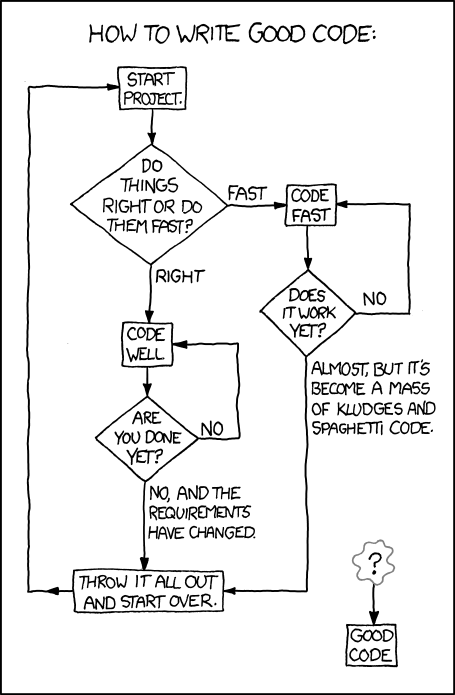
\includegraphics[height=0.9\textheight]{xkcd_good_code}
		
		{\tiny\url{http://xkcd.com/844/}}
	\end{center}
\end{frame}

\begin{frame}{Flowcharts}
	\begin{itemize}
		\pause\item Represent \textbf{control flow} in an algorithm or a computing system
		\pause\item Start at the start, and follow the arrows!
		\pause\item \textbf{Branches} (\texttt{if} statements) are represented as a choice of 2 or more arrows to go down
		\pause\item \textbf{Loops} are represented by the path looping back on itself
		\pause\item Basic \textbf{concurrency} can be represented with ``fork'' and ``join'' points
		\begin{itemize}
			\item Fork: go down multiple arrows simultaneously
			\item Join: wait for multiple incoming arrows to arrive
		\end{itemize}
	\end{itemize}
\end{frame}

\begin{frame}{UML}
	\begin{itemize}
		\pause\item Unified Modeling Language
		\pause\item Defines 14 types of diagram to represent various aspects of computing systems
		\pause\item Activity diagrams: UML version of flowcharts
	\end{itemize}
\end{frame}

\begin{frame}{UML Activity Diagram}
	\begin{columns}
		\begin{column}{0.4\textwidth}
			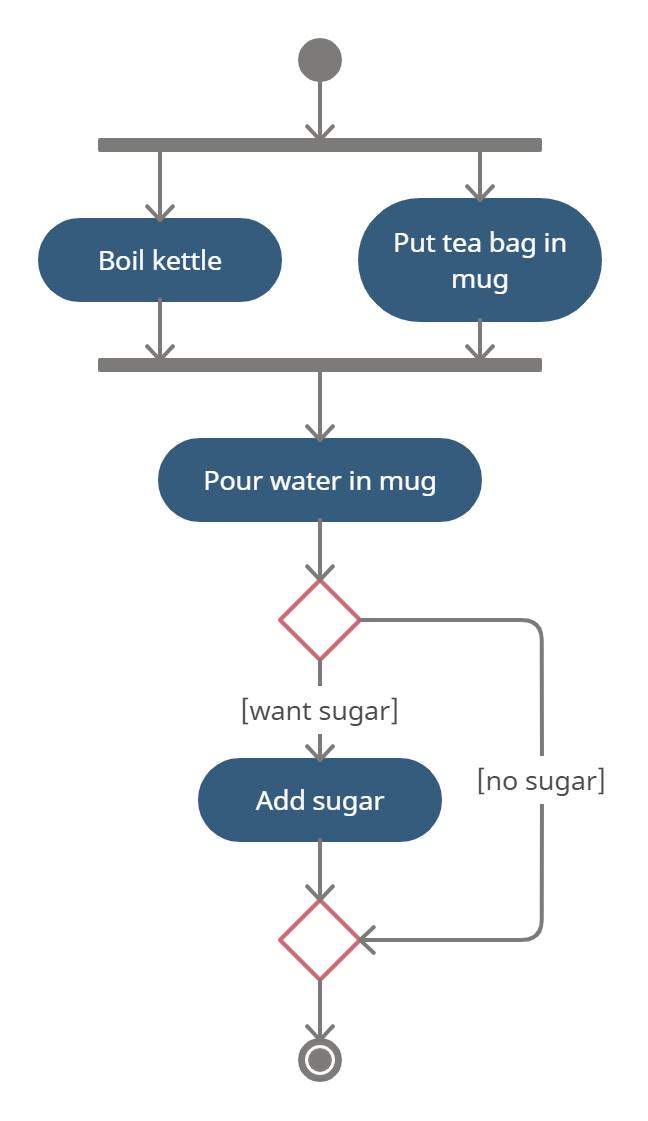
\includegraphics[width=\textwidth]{activity_diagram}
		\end{column}
		\begin{column}{0.58\textwidth}
		\end{column}
	\end{columns}
\end{frame}

\begin{frame}{UML Activity Diagram Symbols}
	\begin{columns}
		\begin{column}{0.4\textwidth}
			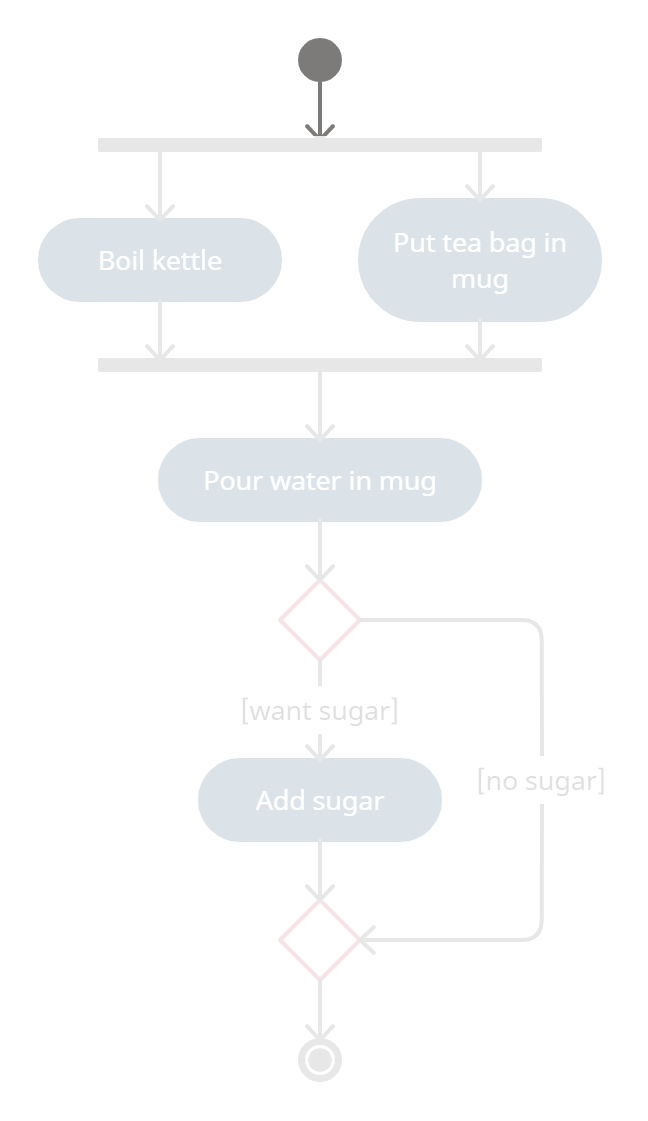
\includegraphics[width=\textwidth]{ad_start}
		\end{column}
		\begin{column}{0.58\textwidth}
			\begin{itemize}
				\pause\item \textbf{Start} node shows where control flow begins
				\pause\item An activity diagram must have exactly one of these!
			\end{itemize}
		\end{column}
	\end{columns}
\end{frame}

\begin{frame}{UML Activity Diagram Symbols}
	\begin{columns}
		\begin{column}{0.4\textwidth}
			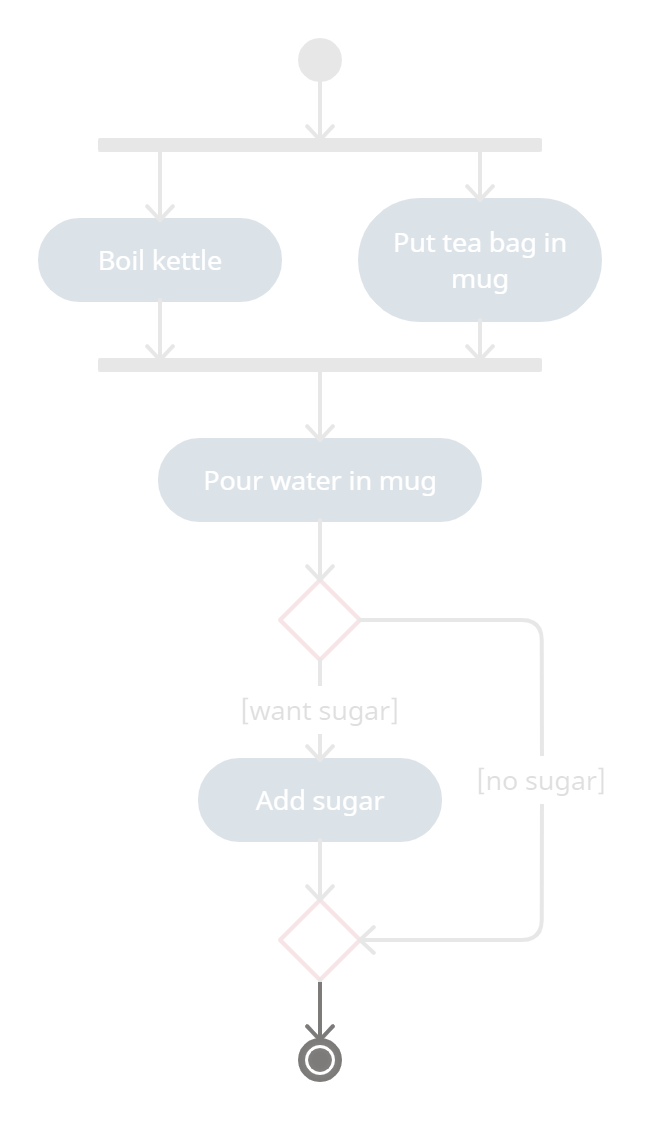
\includegraphics[width=\textwidth]{ad_end}
		\end{column}
		\begin{column}{0.58\textwidth}
			\begin{itemize}
				\pause\item \textbf{End} node shows where control flow terminates
				\pause\item An activity diagram usually has one of these
			\end{itemize}
		\end{column}
	\end{columns}
\end{frame}

\begin{frame}{UML Activity Diagram Symbols}
	\begin{columns}
		\begin{column}{0.4\textwidth}
			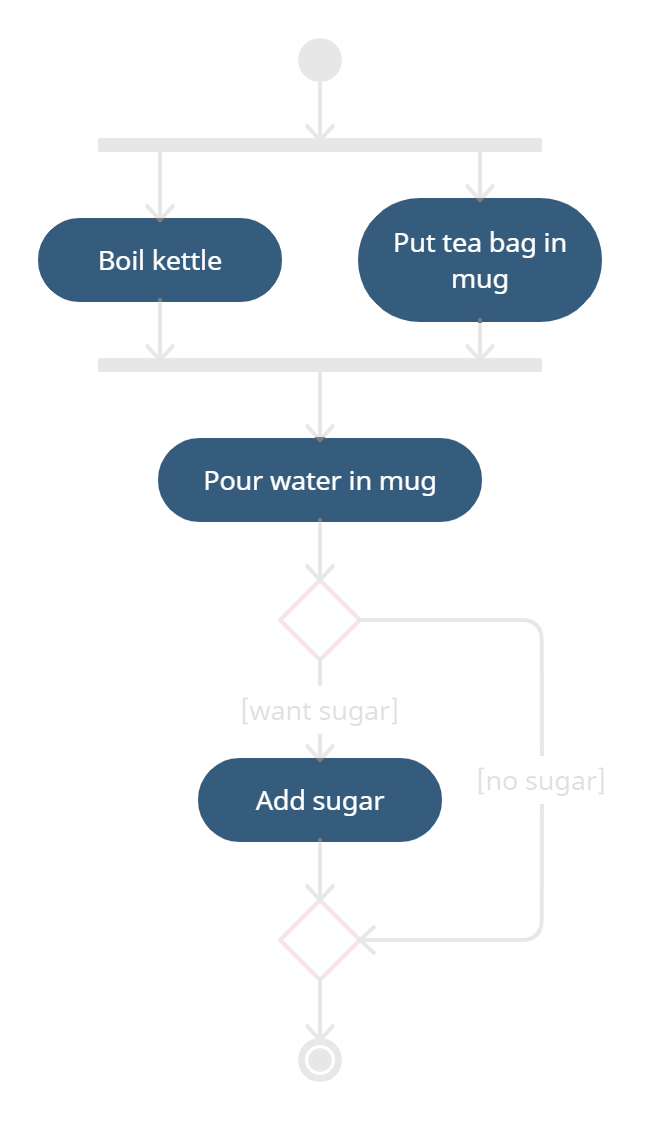
\includegraphics[width=\textwidth]{ad_action}
		\end{column}
		\begin{column}{0.58\textwidth}
			\begin{itemize}
				\pause\item \textbf{Action} or \textbf{activity} nodes describe the operations that are carried out
			\end{itemize}
		\end{column}
	\end{columns}
\end{frame}

\begin{frame}{UML Activity Diagram Symbols}
	\begin{columns}
		\begin{column}{0.4\textwidth}
			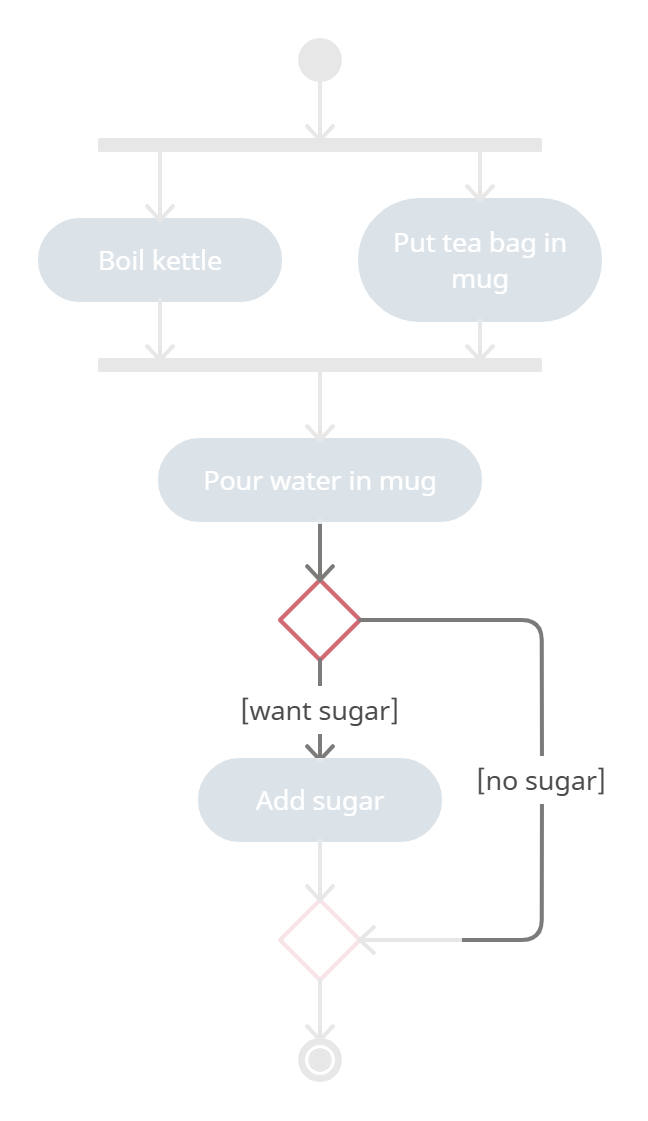
\includegraphics[width=\textwidth]{ad_decision}
		\end{column}
		\begin{column}{0.58\textwidth}
			\begin{itemize}
				\pause\item \textbf{Decision} nodes represent a conditional branch (like an \texttt{if} statement)
				\pause\item Outgoing arrows are labelled with descriptions of the conditions
			\end{itemize}
		\end{column}
	\end{columns}
\end{frame}

\begin{frame}{UML Activity Diagram Symbols}
	\begin{columns}
		\begin{column}{0.4\textwidth}
			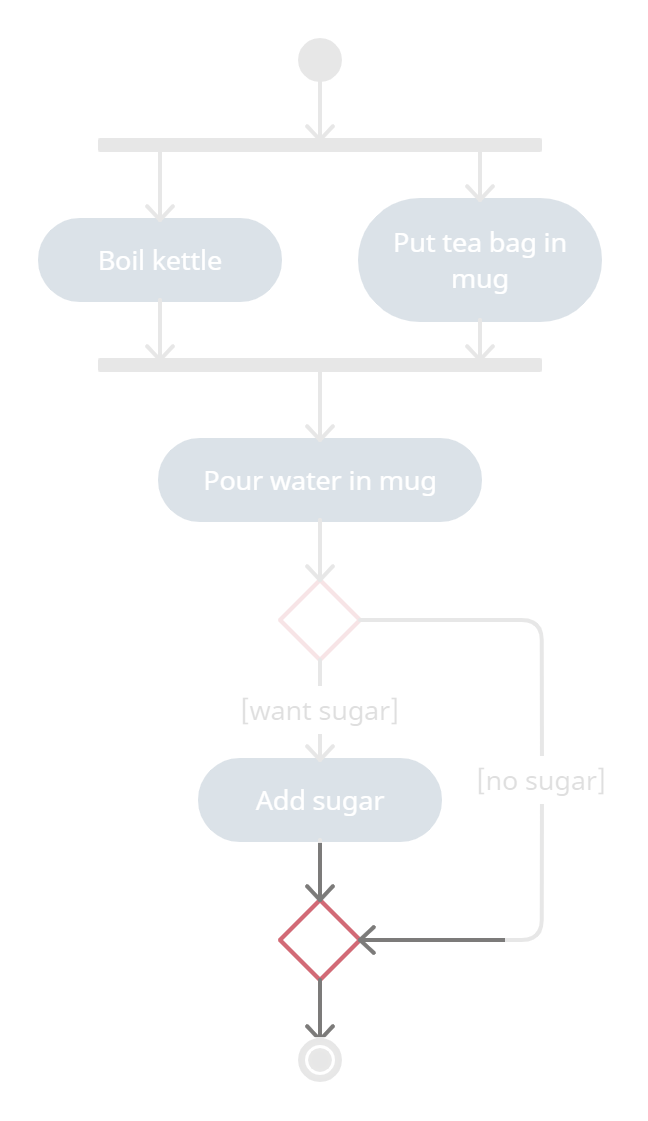
\includegraphics[width=\textwidth]{ad_merge}
		\end{column}
		\begin{column}{0.58\textwidth}
			\begin{itemize}
				\pause\item \textbf{Merge} nodes allow alternative control paths to join together
				\pause\item Commonly used after a decision node
			\end{itemize}
		\end{column}
	\end{columns}
\end{frame}

\begin{frame}{UML Activity Diagram Symbols}
	\begin{columns}
		\begin{column}{0.4\textwidth}
			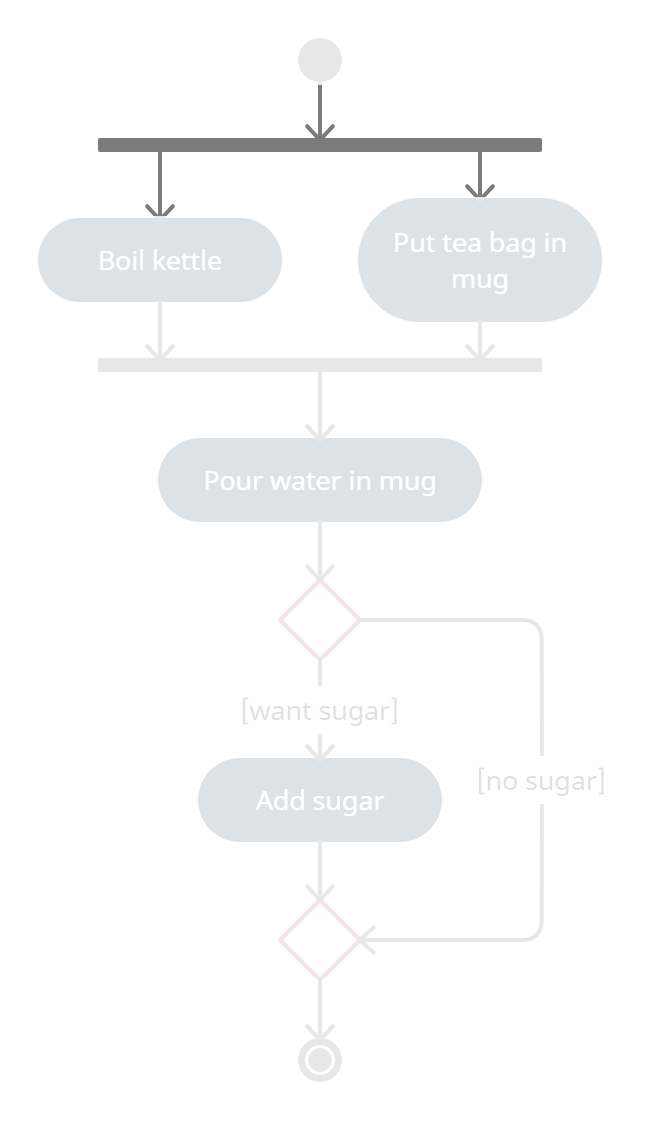
\includegraphics[width=\textwidth]{ad_fork}
		\end{column}
		\begin{column}{0.58\textwidth}
			\begin{itemize}
				\pause\item \textbf{Fork} nodes represent concurrent (parallel) processes
			\end{itemize}
		\end{column}
	\end{columns}
\end{frame}

\begin{frame}{UML Activity Diagram Symbols}
	\begin{columns}
		\begin{column}{0.4\textwidth}
			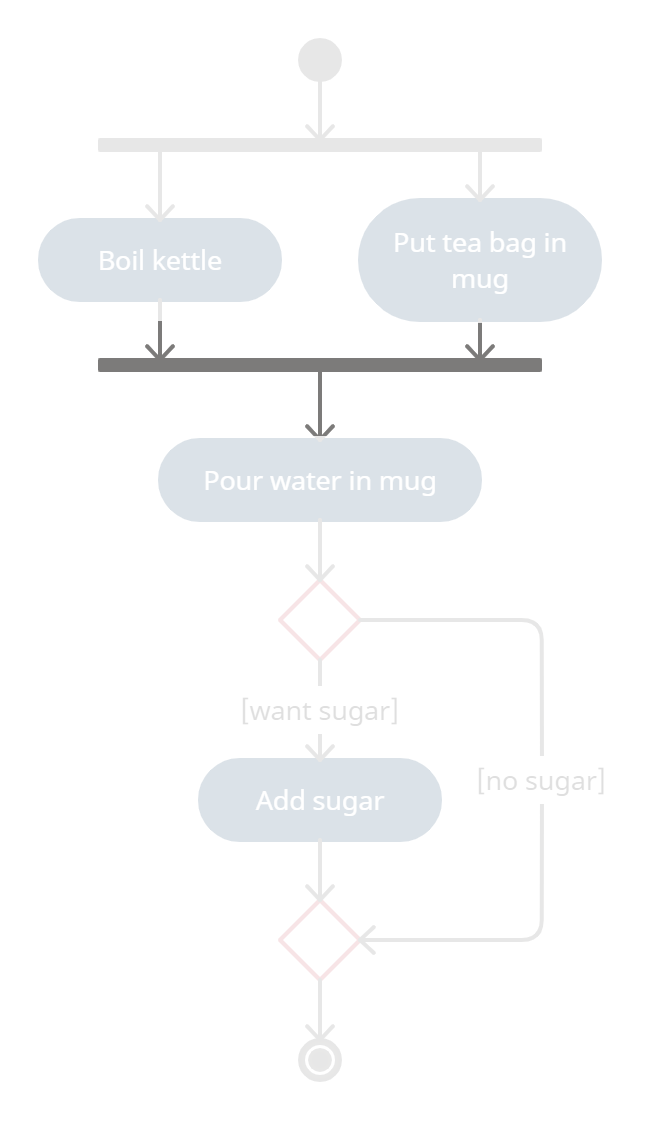
\includegraphics[width=\textwidth]{ad_join}
		\end{column}
		\begin{column}{0.58\textwidth}
			\begin{itemize}
				\pause\item \textbf{Join} nodes allow forked processes to join together again
				\pause\item Control waits until all processes are ready
			\end{itemize}
		\end{column}
	\end{columns}
\end{frame}

\begin{frame}{Swimlanes}
	\begin{center}
		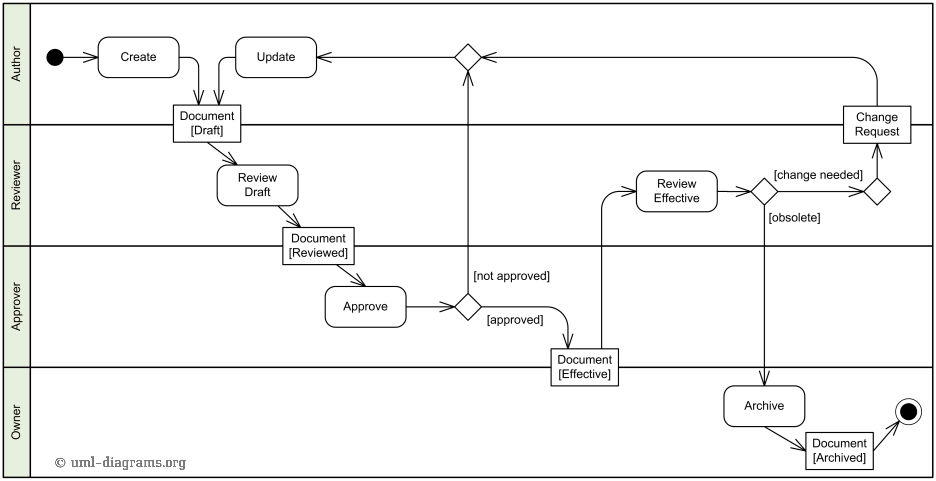
\includegraphics[width=\textwidth]{activity-example-document-management}
	\end{center}
	\begin{itemize}
		\item Allow an activity diagram to represent interacting \textbf{subsystems}
	\end{itemize}
\end{frame}

\begin{frame}{Software for drawing UML diagrams}
	\begin{itemize}
		\item Diagrams.net
		\item Creately
		\item Microsoft Visio
		\item (If you must) any other graphics software
	\end{itemize}
\end{frame}

\begin{frame}{Activity}
	\begin{itemize}
		\item In your \textbf{breakout groups}
		\item \textbf{Draw} an activity diagram for \textbf{logging into Facebook}
		\item (Tip: either use the Teams whiteboard, or screen sharing with remote control, to collaborate on the same diagram)
		\item Include at least two swimlanes: \textbf{the user's browser/device} and \textbf{the Facebook server}
	\end{itemize}
\end{frame}
